\documentclass[1p]{elsarticle_modified}
%\bibliographystyle{elsarticle-num}

%\usepackage[colorlinks]{hyperref}
%\usepackage{abbrmath_seonhwa} %\Abb, \Ascr, \Acal ,\Abf, \Afrak
\usepackage{amsfonts}
\usepackage{amssymb}
\usepackage{amsmath}
\usepackage{amsthm}
\usepackage{scalefnt}
\usepackage{amsbsy}
\usepackage{kotex}
\usepackage{caption}
\usepackage{subfig}
\usepackage{color}
\usepackage{graphicx}
\usepackage{xcolor} %% white, black, red, green, blue, cyan, magenta, yellow
\usepackage{float}
\usepackage{setspace}
\usepackage{hyperref}

\usepackage{tikz}
\usetikzlibrary{arrows}

\usepackage{multirow}
\usepackage{array} % fixed length table
\usepackage{hhline}

%%%%%%%%%%%%%%%%%%%%%
\makeatletter
\renewcommand*\env@matrix[1][\arraystretch]{%
	\edef\arraystretch{#1}%
	\hskip -\arraycolsep
	\let\@ifnextchar\new@ifnextchar
	\array{*\c@MaxMatrixCols c}}
\makeatother %https://tex.stackexchange.com/questions/14071/how-can-i-increase-the-line-spacing-in-a-matrix
%%%%%%%%%%%%%%%

\usepackage[normalem]{ulem}

\newcommand{\msout}[1]{\ifmmode\text{\sout{\ensuremath{#1}}}\else\sout{#1}\fi}
%SOURCE: \msout is \stkout macro in https://tex.stackexchange.com/questions/20609/strikeout-in-math-mode

\newcommand{\cancel}[1]{
	\ifmmode
	{\color{red}\msout{#1}}
	\else
	{\color{red}\sout{#1}}
	\fi
}

\newcommand{\add}[1]{
	{\color{blue}\uwave{#1}}
}

\newcommand{\replace}[2]{
	\ifmmode
	{\color{red}\msout{#1}}{\color{blue}\uwave{#2}}
	\else
	{\color{red}\sout{#1}}{\color{blue}\uwave{#2}}
	\fi
}

\newcommand{\Sol}{\mathcal{S}} %segment
\newcommand{\D}{D} %diagram
\newcommand{\A}{\mathcal{A}} %arc


%%%%%%%%%%%%%%%%%%%%%%%%%%%%%5 test

\def\sl{\operatorname{\textup{SL}}(2,\Cbb)}
\def\psl{\operatorname{\textup{PSL}}(2,\Cbb)}
\def\quan{\mkern 1mu \triangleright \mkern 1mu}

\theoremstyle{definition}
\newtheorem{thm}{Theorem}[section]
\newtheorem{prop}[thm]{Proposition}
\newtheorem{lem}[thm]{Lemma}
\newtheorem{ques}[thm]{Question}
\newtheorem{cor}[thm]{Corollary}
\newtheorem{defn}[thm]{Definition}
\newtheorem{exam}[thm]{Example}
\newtheorem{rmk}[thm]{Remark}
\newtheorem{alg}[thm]{Algorithm}

\newcommand{\I}{\sqrt{-1}}
\begin{document}

%\begin{frontmatter}
%
%\title{Boundary parabolic representations of knots up to 8 crossings}
%
%%% Group authors per affiliation:
%\author{Yunhi Cho} 
%\address{Department of Mathematics, University of Seoul, Seoul, Korea}
%\ead{yhcho@uos.ac.kr}
%
%
%\author{Seonhwa Kim} %\fnref{s_kim}}
%\address{Center for Geometry and Physics, Institute for Basic Science, Pohang, 37673, Korea}
%\ead{ryeona17@ibs.re.kr}
%
%\author{Hyuk Kim}
%\address{Department of Mathematical Sciences, Seoul National University, Seoul 08826, Korea}
%\ead{hyukkim@snu.ac.kr}
%
%\author{Seokbeom Yoon}
%\address{Department of Mathematical Sciences, Seoul National University, Seoul, 08826,  Korea}
%\ead{sbyoon15@snu.ac.kr}
%
%\begin{abstract}
%We find all boundary parabolic representation of knots up to 8 crossings.
%
%\end{abstract}
%\begin{keyword}
%    \MSC[2010] 57M25 
%\end{keyword}
%
%\end{frontmatter}

%\linenumbers
%\tableofcontents
%
\newcommand\colored[1]{\textcolor{white}{\rule[-0.35ex]{0.8em}{1.4ex}}\kern-0.8em\color{red} #1}%
%\newcommand\colored[1]{\textcolor{white}{ #1}\kern-2.17ex	\textcolor{white}{ #1}\kern-1.81ex	\textcolor{white}{ #1}\kern-2.15ex\color{red}#1	}

{\Large $\underline{12a_{0902}~(K12a_{0902})}$}

\setlength{\tabcolsep}{10pt}
\renewcommand{\arraystretch}{1.6}
\vspace{1cm}\begin{tabular}{m{100pt}>{\centering\arraybackslash}m{274pt}}
\multirow{5}{120pt}{
	\centering
	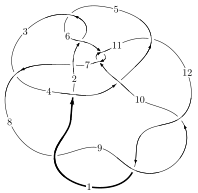
\includegraphics[width=112pt]{../../../GIT/diagram.site/Diagrams/png/1703_12a_0902.png}\\
\ \ \ A knot diagram\footnotemark}&
\allowdisplaybreaks
\textbf{Linearized knot diagam} \\
\cline{2-2}
 &
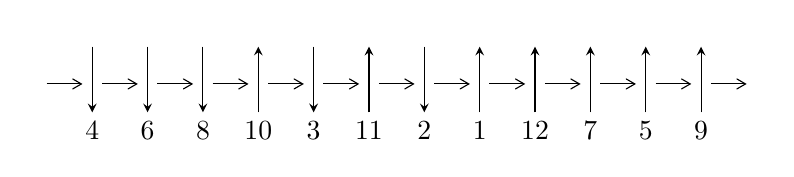
\begin{tikzpicture}[x=20pt, y=17pt]
	% nodes
	\node (C0) at (0, 0) {};
	\node (C1) at (1, 0) {};
	\node (C1U) at (1, +1) {};
	\node (C1D) at (1, -1) {4};

	\node (C2) at (2, 0) {};
	\node (C2U) at (2, +1) {};
	\node (C2D) at (2, -1) {6};

	\node (C3) at (3, 0) {};
	\node (C3U) at (3, +1) {};
	\node (C3D) at (3, -1) {8};

	\node (C4) at (4, 0) {};
	\node (C4U) at (4, +1) {};
	\node (C4D) at (4, -1) {10};

	\node (C5) at (5, 0) {};
	\node (C5U) at (5, +1) {};
	\node (C5D) at (5, -1) {3};

	\node (C6) at (6, 0) {};
	\node (C6U) at (6, +1) {};
	\node (C6D) at (6, -1) {11};

	\node (C7) at (7, 0) {};
	\node (C7U) at (7, +1) {};
	\node (C7D) at (7, -1) {2};

	\node (C8) at (8, 0) {};
	\node (C8U) at (8, +1) {};
	\node (C8D) at (8, -1) {1};

	\node (C9) at (9, 0) {};
	\node (C9U) at (9, +1) {};
	\node (C9D) at (9, -1) {12};

	\node (C10) at (10, 0) {};
	\node (C10U) at (10, +1) {};
	\node (C10D) at (10, -1) {7};

	\node (C11) at (11, 0) {};
	\node (C11U) at (11, +1) {};
	\node (C11D) at (11, -1) {5};

	\node (C12) at (12, 0) {};
	\node (C12U) at (12, +1) {};
	\node (C12D) at (12, -1) {9};
	\node (C13) at (13, 0) {};

	% arrows
	\draw[->,>={angle 60}]
	(C0) edge (C1) (C1) edge (C2) (C2) edge (C3) (C3) edge (C4) (C4) edge (C5) (C5) edge (C6) (C6) edge (C7) (C7) edge (C8) (C8) edge (C9) (C9) edge (C10) (C10) edge (C11) (C11) edge (C12) (C12) edge (C13) ;	\draw[->,>=stealth]
	(C1U) edge (C1D) (C2U) edge (C2D) (C3U) edge (C3D) (C4D) edge (C4U) (C5U) edge (C5D) (C6D) edge (C6U) (C7U) edge (C7D) (C8D) edge (C8U) (C9D) edge (C9U) (C10D) edge (C10U) (C11D) edge (C11U) (C12D) edge (C12U) ;
	\end{tikzpicture} \\
\hhline{~~} \\& 
\textbf{Solving Sequence} \\ \cline{2-2} 
 &
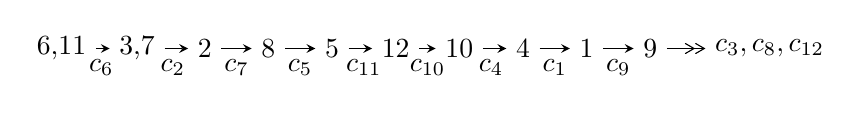
\begin{tikzpicture}[x=23pt, y=7pt]
	% node
	\node (A0) at (-1/8, 0) {6,11};
	\node (A1) at (17/16, 0) {3,7};
	\node (A2) at (17/8, 0) {2};
	\node (A3) at (25/8, 0) {8};
	\node (A4) at (33/8, 0) {5};
	\node (A5) at (41/8, 0) {12};
	\node (A6) at (49/8, 0) {10};
	\node (A7) at (57/8, 0) {4};
	\node (A8) at (65/8, 0) {1};
	\node (A9) at (73/8, 0) {9};
	\node (C1) at (1/2, -1) {$c_{6}$};
	\node (C2) at (13/8, -1) {$c_{2}$};
	\node (C3) at (21/8, -1) {$c_{7}$};
	\node (C4) at (29/8, -1) {$c_{5}$};
	\node (C5) at (37/8, -1) {$c_{11}$};
	\node (C6) at (45/8, -1) {$c_{10}$};
	\node (C7) at (53/8, -1) {$c_{4}$};
	\node (C8) at (61/8, -1) {$c_{1}$};
	\node (C9) at (69/8, -1) {$c_{9}$};
	\node (A10) at (11, 0) {$c_{3},c_{8},c_{12}$};

	% edge
	\draw[->,>=stealth]	
	(A0) edge (A1) (A1) edge (A2) (A2) edge (A3) (A3) edge (A4) (A4) edge (A5) (A5) edge (A6) (A6) edge (A7) (A7) edge (A8) (A8) edge (A9) ;
	\draw[->>,>={angle 60}]	
	(A9) edge (A10);
\end{tikzpicture} \\ 

\end{tabular} \\

\footnotetext{
The image of knot diagram is generated by the software ``\textbf{Draw programme}" developed by Andrew Bartholomew(\url{http://www.layer8.co.uk/maths/draw/index.htm\#Running-draw}), where we modified some parts for our purpose(\url{https://github.com/CATsTAILs/LinksPainter}).
}\phantom \\ \newline 
\centering \textbf{Ideals for irreducible components\footnotemark of $X_{\text{par}}$} 
 
\begin{align*}
I^u_{1}&=\langle 
2.28807\times10^{579} u^{141}-6.43625\times10^{579} u^{140}+\cdots+1.05243\times10^{581} b-1.13630\times10^{583},\\
\phantom{I^u_{1}}&\phantom{= \langle  }-5.53214\times10^{582} u^{141}-3.86140\times10^{582} u^{140}+\cdots+2.97837\times10^{583} a+3.74063\times10^{585},\\
\phantom{I^u_{1}}&\phantom{= \langle  }u^{142}+u^{141}+\cdots-433 u+566\rangle \\
I^u_{2}&=\langle 
-2.57367\times10^{19} u^{35}+4.86277\times10^{19} u^{34}+\cdots+2.01550\times10^{18} b-8.20022\times10^{17},\\
\phantom{I^u_{2}}&\phantom{= \langle  }6.09631\times10^{19} u^{35}-1.33362\times10^{20} u^{34}+\cdots+2.01550\times10^{18} a+1.44484\times10^{18},\;u^{36}-2 u^{35}+\cdots+14 u^2+1\rangle \\
\\
\end{align*}
\raggedright * 2 irreducible components of $\dim_{\mathbb{C}}=0$, with total 178 representations.\\
\footnotetext{All coefficients of polynomials are rational numbers. But the coefficients are sometimes approximated in decimal forms when there is not enough margin.}
\newpage
\renewcommand{\arraystretch}{1}
\centering \section*{I. $I^u_{1}= \langle 2.29\times10^{579} u^{141}-6.44\times10^{579} u^{140}+\cdots+1.05\times10^{581} b-1.14\times10^{583},\;-5.53\times10^{582} u^{141}-3.86\times10^{582} u^{140}+\cdots+2.98\times10^{583} a+3.74\times10^{585},\;u^{142}+u^{141}+\cdots-433 u+566 \rangle$}
\flushleft \textbf{(i) Arc colorings}\\
\begin{tabular}{m{7pt} m{180pt} m{7pt} m{180pt} }
\flushright $a_{6}=$&$\begin{pmatrix}1\\0\end{pmatrix}$ \\
\flushright $a_{11}=$&$\begin{pmatrix}0\\u\end{pmatrix}$ \\
\flushright $a_{3}=$&$\begin{pmatrix}0.185744 u^{141}+0.129648 u^{140}+\cdots+322.302 u-125.593\\-0.0217409 u^{141}+0.0611562 u^{140}+\cdots-118.415 u+107.969\end{pmatrix}$ \\
\flushright $a_{7}=$&$\begin{pmatrix}1\\- u^2\end{pmatrix}$ \\
\flushright $a_{2}=$&$\begin{pmatrix}0.164003 u^{141}+0.190804 u^{140}+\cdots+203.887 u-17.6243\\-0.0217409 u^{141}+0.0611562 u^{140}+\cdots-118.415 u+107.969\end{pmatrix}$ \\
\flushright $a_{8}=$&$\begin{pmatrix}0.309742 u^{141}+0.350704 u^{140}+\cdots+493.397 u-53.3774\\-0.0719401 u^{141}-0.0810056 u^{140}+\cdots-131.013 u+13.3389\end{pmatrix}$ \\
\flushright $a_{5}=$&$\begin{pmatrix}-0.121598 u^{141}-0.0533193 u^{140}+\cdots-327.614 u+128.023\\0.0891752 u^{141}+0.159360 u^{140}+\cdots+52.7069 u+65.0312\end{pmatrix}$ \\
\flushright $a_{12}=$&$\begin{pmatrix}0.293005 u^{141}+0.169552 u^{140}+\cdots+378.798 u-149.784\\-0.0739083 u^{141}-0.0139821 u^{140}+\cdots-108.232 u+84.0302\end{pmatrix}$ \\
\flushright $a_{10}=$&$\begin{pmatrix}- u\\u^3+u\end{pmatrix}$ \\
\flushright $a_{4}=$&$\begin{pmatrix}-0.106030 u^{141}+0.0168797 u^{140}+\cdots-381.916 u+195.461\\0.0887523 u^{141}+0.131058 u^{140}+\cdots+92.1652 u+28.5140\end{pmatrix}$ \\
\flushright $a_{1}=$&$\begin{pmatrix}0.0525750 u^{141}-0.0742782 u^{140}+\cdots+367.180 u-194.571\\0.0505938 u^{141}+0.117664 u^{140}+\cdots-22.8007 u+72.9937\end{pmatrix}$ \\
\flushright $a_{9}=$&$\begin{pmatrix}-0.470709 u^{141}-0.618514 u^{140}+\cdots-641.784 u-141.596\\0.0411816 u^{141}+0.125305 u^{140}+\cdots+9.96569 u+101.141\end{pmatrix}$\\&\end{tabular}
\flushleft \textbf{(ii) Obstruction class $= -1$}\\~\\
\flushleft \textbf{(iii) Cusp Shapes $= -0.326552 u^{141}-0.235065 u^{140}+\cdots-376.096 u+126.428$}\\~\\
\newpage\renewcommand{\arraystretch}{1}
\flushleft \textbf{(iv) u-Polynomials at the component}\newline \\
\begin{tabular}{m{50pt}|m{274pt}}
Crossings & \hspace{64pt}u-Polynomials at each crossing \\
\hline $$\begin{aligned}c_{1}\end{aligned}$$&$\begin{aligned}
&u^{142}-11 u^{141}+\cdots+60356 u+9829
\end{aligned}$\\
\hline $$\begin{aligned}c_{2},c_{5}\end{aligned}$$&$\begin{aligned}
&u^{142}+10 u^{141}+\cdots-30698 u+7239
\end{aligned}$\\
\hline $$\begin{aligned}c_{3}\end{aligned}$$&$\begin{aligned}
&u^{142}- u^{141}+\cdots-5976125 u+475354
\end{aligned}$\\
\hline $$\begin{aligned}c_{4}\end{aligned}$$&$\begin{aligned}
&u^{142}- u^{141}+\cdots+2114842 u+213833
\end{aligned}$\\
\hline $$\begin{aligned}c_{6},c_{10}\end{aligned}$$&$\begin{aligned}
&u^{142}+u^{141}+\cdots-433 u+566
\end{aligned}$\\
\hline $$\begin{aligned}c_{7}\end{aligned}$$&$\begin{aligned}
&u^{142}- u^{141}+\cdots-1090932 u+74313
\end{aligned}$\\
\hline $$\begin{aligned}c_{8},c_{9},c_{12}\end{aligned}$$&$\begin{aligned}
&u^{142}+3 u^{141}+\cdots+11 u+3
\end{aligned}$\\
\hline $$\begin{aligned}c_{11}\end{aligned}$$&$\begin{aligned}
&u^{142}+u^{141}+\cdots+31729814 u+9330071
\end{aligned}$\\
\hline
\end{tabular}\\~\\
\newpage\renewcommand{\arraystretch}{1}
\flushleft \textbf{(v) Riley Polynomials at the component}\newline \\
\begin{tabular}{m{50pt}|m{274pt}}
Crossings & \hspace{64pt}Riley Polynomials at each crossing \\
\hline $$\begin{aligned}c_{1}\end{aligned}$$&$\begin{aligned}
&y^{142}-33 y^{141}+\cdots-4656904666 y+96609241
\end{aligned}$\\
\hline $$\begin{aligned}c_{2},c_{5}\end{aligned}$$&$\begin{aligned}
&y^{142}+72 y^{141}+\cdots+1964047862 y+52403121
\end{aligned}$\\
\hline $$\begin{aligned}c_{3}\end{aligned}$$&$\begin{aligned}
&y^{142}-37 y^{141}+\cdots-14479019050013 y+225961425316
\end{aligned}$\\
\hline $$\begin{aligned}c_{4}\end{aligned}$$&$\begin{aligned}
&y^{142}+41 y^{141}+\cdots+1108048823382 y+45724551889
\end{aligned}$\\
\hline $$\begin{aligned}c_{6},c_{10}\end{aligned}$$&$\begin{aligned}
&y^{142}+75 y^{141}+\cdots+11660023 y+320356
\end{aligned}$\\
\hline $$\begin{aligned}c_{7}\end{aligned}$$&$\begin{aligned}
&y^{142}+27 y^{141}+\cdots+321386954580 y+5522421969
\end{aligned}$\\
\hline $$\begin{aligned}c_{8},c_{9},c_{12}\end{aligned}$$&$\begin{aligned}
&y^{142}+147 y^{141}+\cdots+239 y+9
\end{aligned}$\\
\hline $$\begin{aligned}c_{11}\end{aligned}$$&$\begin{aligned}
&y^{142}+45 y^{141}+\cdots+2490029141421586 y+87050224865041
\end{aligned}$\\
\hline
\end{tabular}\\~\\
\newpage\flushleft \textbf{(vi) Complex Volumes and Cusp Shapes}
$$\begin{array}{c|c|c}  
\text{Solutions to }I^u_{1}& \I (\text{vol} + \sqrt{-1}CS) & \text{Cusp shape}\\
 \hline 
\begin{aligned}
u &= -0.478669 + 0.856250 I \\
a &= \phantom{-}1.33220 - 0.64590 I \\
b &= \phantom{-}0.383497 + 1.146310 I\end{aligned}
 & \phantom{-}3.46210 + 0.57689 I & \phantom{-0.000000 } 0 \\ \hline\begin{aligned}
u &= -0.478669 - 0.856250 I \\
a &= \phantom{-}1.33220 + 0.64590 I \\
b &= \phantom{-}0.383497 - 1.146310 I\end{aligned}
 & \phantom{-}3.46210 - 0.57689 I & \phantom{-0.000000 } 0 \\ \hline\begin{aligned}
u &= -0.276069 + 0.983520 I \\
a &= -0.223608 + 0.516278 I \\
b &= -1.254720 + 0.327774 I\end{aligned}
 & -4.00562 - 0.90784 I & \phantom{-0.000000 } 0 \\ \hline\begin{aligned}
u &= -0.276069 - 0.983520 I \\
a &= -0.223608 - 0.516278 I \\
b &= -1.254720 - 0.327774 I\end{aligned}
 & -4.00562 + 0.90784 I & \phantom{-0.000000 } 0 \\ \hline\begin{aligned}
u &= \phantom{-}0.587967 + 0.847989 I \\
a &= \phantom{-}1.20752 + 0.85788 I \\
b &= \phantom{-}0.514239 - 0.957313 I\end{aligned}
 & \phantom{-}2.57766 + 3.35143 I & \phantom{-0.000000 } 0 \\ \hline\begin{aligned}
u &= \phantom{-}0.587967 - 0.847989 I \\
a &= \phantom{-}1.20752 - 0.85788 I \\
b &= \phantom{-}0.514239 + 0.957313 I\end{aligned}
 & \phantom{-}2.57766 - 3.35143 I & \phantom{-0.000000 } 0 \\ \hline\begin{aligned}
u &= \phantom{-}0.420975 + 0.862842 I \\
a &= \phantom{-}1.37063 + 0.46303 I \\
b &= \phantom{-}0.254616 - 1.311030 I\end{aligned}
 & -2.54002 - 3.38817 I & \phantom{-0.000000 } 0 \\ \hline\begin{aligned}
u &= \phantom{-}0.420975 - 0.862842 I \\
a &= \phantom{-}1.37063 - 0.46303 I \\
b &= \phantom{-}0.254616 + 1.311030 I\end{aligned}
 & -2.54002 + 3.38817 I & \phantom{-0.000000 } 0 \\ \hline\begin{aligned}
u &= \phantom{-}0.168952 + 1.026210 I \\
a &= -0.356726 + 0.070450 I \\
b &= -1.280580 - 0.362676 I\end{aligned}
 & -4.05586 + 0.44867 I & \phantom{-0.000000 } 0 \\ \hline\begin{aligned}
u &= \phantom{-}0.168952 - 1.026210 I \\
a &= -0.356726 - 0.070450 I \\
b &= -1.280580 + 0.362676 I\end{aligned}
 & -4.05586 - 0.44867 I & \phantom{-0.000000 } 0\\
 \hline 
 \end{array}$$\newpage$$\begin{array}{c|c|c}  
\text{Solutions to }I^u_{1}& \I (\text{vol} + \sqrt{-1}CS) & \text{Cusp shape}\\
 \hline 
\begin{aligned}
u &= \phantom{-}0.305624 + 0.994112 I \\
a &= -0.039538 - 0.797063 I \\
b &= -1.47194 - 0.29326 I\end{aligned}
 & -10.36690 + 0.94731 I & \phantom{-0.000000 } 0 \\ \hline\begin{aligned}
u &= \phantom{-}0.305624 - 0.994112 I \\
a &= -0.039538 + 0.797063 I \\
b &= -1.47194 + 0.29326 I\end{aligned}
 & -10.36690 - 0.94731 I & \phantom{-0.000000 } 0 \\ \hline\begin{aligned}
u &= \phantom{-}0.328331 + 1.000760 I \\
a &= \phantom{-}0.509886 - 0.205943 I \\
b &= -0.978942 - 0.877373 I\end{aligned}
 & -8.45607 - 1.93135 I & \phantom{-0.000000 } 0 \\ \hline\begin{aligned}
u &= \phantom{-}0.328331 - 1.000760 I \\
a &= \phantom{-}0.509886 + 0.205943 I \\
b &= -0.978942 + 0.877373 I\end{aligned}
 & -8.45607 + 1.93135 I & \phantom{-0.000000 } 0 \\ \hline\begin{aligned}
u &= -0.968840 + 0.437352 I \\
a &= -0.244962 + 0.682190 I \\
b &= \phantom{-}0.544550 - 0.862963 I\end{aligned}
 & -5.46124 - 1.69208 I & \phantom{-0.000000 } 0 \\ \hline\begin{aligned}
u &= -0.968840 - 0.437352 I \\
a &= -0.244962 - 0.682190 I \\
b &= \phantom{-}0.544550 + 0.862963 I\end{aligned}
 & -5.46124 + 1.69208 I & \phantom{-0.000000 } 0 \\ \hline\begin{aligned}
u &= -0.107346 + 1.063880 I \\
a &= -0.273242 - 0.295384 I \\
b &= -1.50566 + 0.37213 I\end{aligned}
 & -10.44900 - 0.12490 I & \phantom{-0.000000 } 0 \\ \hline\begin{aligned}
u &= -0.107346 - 1.063880 I \\
a &= -0.273242 + 0.295384 I \\
b &= -1.50566 - 0.37213 I\end{aligned}
 & -10.44900 + 0.12490 I & \phantom{-0.000000 } 0 \\ \hline\begin{aligned}
u &= -1.075090 + 0.049904 I \\
a &= \phantom{-}0.39394 + 1.52869 I \\
b &= -0.171883 - 1.212840 I\end{aligned}
 & \phantom{-}0.09215 - 2.97768 I & \phantom{-0.000000 } 0 \\ \hline\begin{aligned}
u &= -1.075090 - 0.049904 I \\
a &= \phantom{-}0.39394 - 1.52869 I \\
b &= -0.171883 + 1.212840 I\end{aligned}
 & \phantom{-}0.09215 + 2.97768 I & \phantom{-0.000000 } 0\\
 \hline 
 \end{array}$$\newpage$$\begin{array}{c|c|c}  
\text{Solutions to }I^u_{1}& \I (\text{vol} + \sqrt{-1}CS) & \text{Cusp shape}\\
 \hline 
\begin{aligned}
u &= -0.834850 + 0.360564 I \\
a &= \phantom{-}0.67808 + 1.42823 I \\
b &= -0.352030 - 1.133540 I\end{aligned}
 & -2.50415 - 3.84106 I & \phantom{-0.000000 } 0 \\ \hline\begin{aligned}
u &= -0.834850 - 0.360564 I \\
a &= \phantom{-}0.67808 - 1.42823 I \\
b &= -0.352030 + 1.133540 I\end{aligned}
 & -2.50415 + 3.84106 I & \phantom{-0.000000 } 0 \\ \hline\begin{aligned}
u &= \phantom{-}0.532925 + 0.954910 I \\
a &= -0.54452 - 1.54775 I \\
b &= -0.964111 + 0.691845 I\end{aligned}
 & -8.87435 + 4.97515 I & \phantom{-0.000000 } 0 \\ \hline\begin{aligned}
u &= \phantom{-}0.532925 - 0.954910 I \\
a &= -0.54452 + 1.54775 I \\
b &= -0.964111 - 0.691845 I\end{aligned}
 & -8.87435 - 4.97515 I & \phantom{-0.000000 } 0 \\ \hline\begin{aligned}
u &= -0.343797 + 1.058840 I \\
a &= \phantom{-}0.274425 - 0.063970 I \\
b &= -0.774550 + 0.537885 I\end{aligned}
 & -2.27256 + 0.30412 I & \phantom{-0.000000 } 0 \\ \hline\begin{aligned}
u &= -0.343797 - 1.058840 I \\
a &= \phantom{-}0.274425 + 0.063970 I \\
b &= -0.774550 - 0.537885 I\end{aligned}
 & -2.27256 - 0.30412 I & \phantom{-0.000000 } 0 \\ \hline\begin{aligned}
u &= -0.718421 + 0.515010 I \\
a &= \phantom{-}1.11405 - 1.55879 I \\
b &= \phantom{-}0.753041 + 0.772121 I\end{aligned}
 & -5.89549 - 6.63684 I & \phantom{-0.000000 } 0 \\ \hline\begin{aligned}
u &= -0.718421 - 0.515010 I \\
a &= \phantom{-}1.11405 + 1.55879 I \\
b &= \phantom{-}0.753041 - 0.772121 I\end{aligned}
 & -5.89549 + 6.63684 I & \phantom{-0.000000 } 0 \\ \hline\begin{aligned}
u &= -0.908635 + 0.651617 I \\
a &= -0.20098 + 1.66515 I \\
b &= -0.200393 - 0.692894 I\end{aligned}
 & -1.00289 - 4.26111 I & \phantom{-0.000000 } 0 \\ \hline\begin{aligned}
u &= -0.908635 - 0.651617 I \\
a &= -0.20098 - 1.66515 I \\
b &= -0.200393 + 0.692894 I\end{aligned}
 & -1.00289 + 4.26111 I & \phantom{-0.000000 } 0\\
 \hline 
 \end{array}$$\newpage$$\begin{array}{c|c|c}  
\text{Solutions to }I^u_{1}& \I (\text{vol} + \sqrt{-1}CS) & \text{Cusp shape}\\
 \hline 
\begin{aligned}
u &= \phantom{-}0.588083 + 0.649256 I \\
a &= -0.026913 - 0.970820 I \\
b &= \phantom{-}0.196803 + 1.199740 I\end{aligned}
 & \phantom{-}3.16495 + 1.28532 I & \phantom{-0.000000 } 0 \\ \hline\begin{aligned}
u &= \phantom{-}0.588083 - 0.649256 I \\
a &= -0.026913 + 0.970820 I \\
b &= \phantom{-}0.196803 - 1.199740 I\end{aligned}
 & \phantom{-}3.16495 - 1.28532 I & \phantom{-0.000000 } 0 \\ \hline\begin{aligned}
u &= \phantom{-}0.437260 + 1.051100 I \\
a &= -1.75375 - 0.97756 I \\
b &= -0.402824 + 1.320210 I\end{aligned}
 & -2.92869 + 8.77702 I & \phantom{-0.000000 } 0 \\ \hline\begin{aligned}
u &= \phantom{-}0.437260 - 1.051100 I \\
a &= -1.75375 + 0.97756 I \\
b &= -0.402824 - 1.320210 I\end{aligned}
 & -2.92869 - 8.77702 I & \phantom{-0.000000 } 0 \\ \hline\begin{aligned}
u &= \phantom{-}0.003428 + 0.860712 I \\
a &= -1.09628 - 0.92751 I \\
b &= -0.88457 + 1.13243 I\end{aligned}
 & -7.57932 + 3.21423 I & \phantom{-0.000000 } 0 \\ \hline\begin{aligned}
u &= \phantom{-}0.003428 - 0.860712 I \\
a &= -1.09628 + 0.92751 I \\
b &= -0.88457 - 1.13243 I\end{aligned}
 & -7.57932 - 3.21423 I & \phantom{-0.000000 } 0 \\ \hline\begin{aligned}
u &= -0.358491 + 1.089620 I \\
a &= -1.61364 + 0.32071 I \\
b &= -0.402768 - 1.118320 I\end{aligned}
 & \phantom{-}1.82183 - 6.06054 I & \phantom{-0.000000 } 0 \\ \hline\begin{aligned}
u &= -0.358491 - 1.089620 I \\
a &= -1.61364 - 0.32071 I \\
b &= -0.402768 + 1.118320 I\end{aligned}
 & \phantom{-}1.82183 + 6.06054 I & \phantom{-0.000000 } 0 \\ \hline\begin{aligned}
u &= \phantom{-}1.143980 + 0.138090 I \\
a &= \phantom{-}0.46738 + 1.42871 I \\
b &= \phantom{-}0.452265 - 0.680884 I\end{aligned}
 & \phantom{-}1.57594 + 1.20217 I & \phantom{-0.000000 } 0 \\ \hline\begin{aligned}
u &= \phantom{-}1.143980 - 0.138090 I \\
a &= \phantom{-}0.46738 - 1.42871 I \\
b &= \phantom{-}0.452265 + 0.680884 I\end{aligned}
 & \phantom{-}1.57594 - 1.20217 I & \phantom{-0.000000 } 0\\
 \hline 
 \end{array}$$\newpage$$\begin{array}{c|c|c}  
\text{Solutions to }I^u_{1}& \I (\text{vol} + \sqrt{-1}CS) & \text{Cusp shape}\\
 \hline 
\begin{aligned}
u &= \phantom{-}0.271997 + 1.128510 I \\
a &= -1.244120 + 0.524267 I \\
b &= -0.342755 + 0.875789 I\end{aligned}
 & -0.94220 + 2.37666 I & \phantom{-0.000000 } 0 \\ \hline\begin{aligned}
u &= \phantom{-}0.271997 - 1.128510 I \\
a &= -1.244120 - 0.524267 I \\
b &= -0.342755 - 0.875789 I\end{aligned}
 & -0.94220 - 2.37666 I & \phantom{-0.000000 } 0 \\ \hline\begin{aligned}
u &= \phantom{-}0.292494 + 0.785928 I \\
a &= -0.509142 - 1.181730 I \\
b &= -0.03316 + 1.72308 I\end{aligned}
 & -2.10987 + 6.56452 I & \phantom{-0.000000 } 0 \\ \hline\begin{aligned}
u &= \phantom{-}0.292494 - 0.785928 I \\
a &= -0.509142 + 1.181730 I \\
b &= -0.03316 - 1.72308 I\end{aligned}
 & -2.10987 - 6.56452 I & \phantom{-0.000000 } 0 \\ \hline\begin{aligned}
u &= \phantom{-}0.289860 + 1.155650 I \\
a &= -0.067496 + 0.212863 I \\
b &= -0.740555 + 0.018184 I\end{aligned}
 & -2.68159 + 2.57576 I & \phantom{-0.000000 } 0 \\ \hline\begin{aligned}
u &= \phantom{-}0.289860 - 1.155650 I \\
a &= -0.067496 - 0.212863 I \\
b &= -0.740555 - 0.018184 I\end{aligned}
 & -2.68159 - 2.57576 I & \phantom{-0.000000 } 0 \\ \hline\begin{aligned}
u &= -0.384045 + 1.134370 I \\
a &= \phantom{-}0.98934 - 1.94180 I \\
b &= \phantom{-}0.426980 + 1.102130 I\end{aligned}
 & -9.63220 - 9.37220 I & \phantom{-0.000000 } 0 \\ \hline\begin{aligned}
u &= -0.384045 - 1.134370 I \\
a &= \phantom{-}0.98934 + 1.94180 I \\
b &= \phantom{-}0.426980 - 1.102130 I\end{aligned}
 & -9.63220 + 9.37220 I & \phantom{-0.000000 } 0 \\ \hline\begin{aligned}
u &= \phantom{-}0.590506 + 1.044010 I \\
a &= \phantom{-}1.252460 + 0.627862 I \\
b &= \phantom{-}0.010668 - 0.799440 I\end{aligned}
 & \phantom{-}0.87521 + 2.04600 I & \phantom{-0.000000 } 0 \\ \hline\begin{aligned}
u &= \phantom{-}0.590506 - 1.044010 I \\
a &= \phantom{-}1.252460 - 0.627862 I \\
b &= \phantom{-}0.010668 + 0.799440 I\end{aligned}
 & \phantom{-}0.87521 - 2.04600 I & \phantom{-0.000000 } 0\\
 \hline 
 \end{array}$$\newpage$$\begin{array}{c|c|c}  
\text{Solutions to }I^u_{1}& \I (\text{vol} + \sqrt{-1}CS) & \text{Cusp shape}\\
 \hline 
\begin{aligned}
u &= -0.368091 + 0.707655 I \\
a &= -0.315007 + 1.177230 I \\
b &= \phantom{-}0.05498 - 1.51104 I\end{aligned}
 & \phantom{-}4.01740 - 4.28704 I & \phantom{-0.000000 } 0 \\ \hline\begin{aligned}
u &= -0.368091 - 0.707655 I \\
a &= -0.315007 - 1.177230 I \\
b &= \phantom{-}0.05498 + 1.51104 I\end{aligned}
 & \phantom{-}4.01740 + 4.28704 I & \phantom{-0.000000 } 0 \\ \hline\begin{aligned}
u &= -0.637298 + 1.022940 I \\
a &= \phantom{-}1.38467 - 0.52036 I \\
b &= -0.164880 + 0.719875 I\end{aligned}
 & -4.34036 - 1.57855 I & \phantom{-0.000000 } 0 \\ \hline\begin{aligned}
u &= -0.637298 - 1.022940 I \\
a &= \phantom{-}1.38467 + 0.52036 I \\
b &= -0.164880 - 0.719875 I\end{aligned}
 & -4.34036 + 1.57855 I & \phantom{-0.000000 } 0 \\ \hline\begin{aligned}
u &= -0.559655 + 0.560349 I \\
a &= \phantom{-}0.824163 + 0.312751 I \\
b &= -0.070009 - 0.359810 I\end{aligned}
 & -4.46226 - 2.06361 I & \phantom{-0.000000 } 0 \\ \hline\begin{aligned}
u &= -0.559655 - 0.560349 I \\
a &= \phantom{-}0.824163 - 0.312751 I \\
b &= -0.070009 + 0.359810 I\end{aligned}
 & -4.46226 + 2.06361 I & \phantom{-0.000000 } 0 \\ \hline\begin{aligned}
u &= \phantom{-}0.673809 + 0.410469 I \\
a &= \phantom{-}1.13725 + 1.56194 I \\
b &= -0.566301 - 1.174990 I\end{aligned}
 & -4.78229 - 3.89551 I & \phantom{-0.000000 } 0 \\ \hline\begin{aligned}
u &= \phantom{-}0.673809 - 0.410469 I \\
a &= \phantom{-}1.13725 - 1.56194 I \\
b &= -0.566301 + 1.174990 I\end{aligned}
 & -4.78229 + 3.89551 I & \phantom{-0.000000 } 0 \\ \hline\begin{aligned}
u &= -0.720671 + 0.320211 I \\
a &= \phantom{-}0.76744 - 1.53883 I \\
b &= -0.377558 + 1.169930 I\end{aligned}
 & \phantom{-}1.63882 + 2.84244 I & \phantom{-0.000000 } 0 \\ \hline\begin{aligned}
u &= -0.720671 - 0.320211 I \\
a &= \phantom{-}0.76744 + 1.53883 I \\
b &= -0.377558 - 1.169930 I\end{aligned}
 & \phantom{-}1.63882 - 2.84244 I & \phantom{-0.000000 } 0\\
 \hline 
 \end{array}$$\newpage$$\begin{array}{c|c|c}  
\text{Solutions to }I^u_{1}& \I (\text{vol} + \sqrt{-1}CS) & \text{Cusp shape}\\
 \hline 
\begin{aligned}
u &= \phantom{-}0.038408 + 0.781028 I \\
a &= -1.97752 + 0.88211 I \\
b &= -0.523972 - 0.860480 I\end{aligned}
 & -0.661106 - 1.168450 I & \phantom{-0.000000 } 0 \\ \hline\begin{aligned}
u &= \phantom{-}0.038408 - 0.781028 I \\
a &= -1.97752 - 0.88211 I \\
b &= -0.523972 + 0.860480 I\end{aligned}
 & -0.661106 + 1.168450 I & \phantom{-0.000000 } 0 \\ \hline\begin{aligned}
u &= \phantom{-}0.552073 + 1.085980 I \\
a &= -1.00678 - 1.61348 I \\
b &= -0.77923 + 1.38683 I\end{aligned}
 & -6.77196 + 8.65975 I & \phantom{-0.000000 } 0 \\ \hline\begin{aligned}
u &= \phantom{-}0.552073 - 1.085980 I \\
a &= -1.00678 + 1.61348 I \\
b &= -0.77923 - 1.38683 I\end{aligned}
 & -6.77196 - 8.65975 I & \phantom{-0.000000 } 0 \\ \hline\begin{aligned}
u &= \phantom{-}1.176740 + 0.317476 I \\
a &= -0.421676 - 1.297270 I \\
b &= \phantom{-}0.557082 + 1.188040 I\end{aligned}
 & -4.38743 - 12.66050 I & \phantom{-0.000000 } 0 \\ \hline\begin{aligned}
u &= \phantom{-}1.176740 - 0.317476 I \\
a &= -0.421676 + 1.297270 I \\
b &= \phantom{-}0.557082 - 1.188040 I\end{aligned}
 & -4.38743 + 12.66050 I & \phantom{-0.000000 } 0 \\ \hline\begin{aligned}
u &= \phantom{-}0.746465 + 0.229567 I \\
a &= \phantom{-}0.49746 - 1.46801 I \\
b &= -0.255192 + 1.180850 I\end{aligned}
 & \phantom{-}3.01026 + 2.97423 I & \phantom{-0.000000 } 0 \\ \hline\begin{aligned}
u &= \phantom{-}0.746465 - 0.229567 I \\
a &= \phantom{-}0.49746 + 1.46801 I \\
b &= -0.255192 - 1.180850 I\end{aligned}
 & \phantom{-}3.01026 - 2.97423 I & \phantom{-0.000000 } 0 \\ \hline\begin{aligned}
u &= -0.235899 + 1.198680 I \\
a &= -0.157627 - 0.037888 I \\
b &= -1.107410 - 0.397698 I\end{aligned}
 & -9.58024 - 3.78253 I & \phantom{-0.000000 } 0 \\ \hline\begin{aligned}
u &= -0.235899 - 1.198680 I \\
a &= -0.157627 + 0.037888 I \\
b &= -1.107410 + 0.397698 I\end{aligned}
 & -9.58024 + 3.78253 I & \phantom{-0.000000 } 0\\
 \hline 
 \end{array}$$\newpage$$\begin{array}{c|c|c}  
\text{Solutions to }I^u_{1}& \I (\text{vol} + \sqrt{-1}CS) & \text{Cusp shape}\\
 \hline 
\begin{aligned}
u &= \phantom{-}0.366840 + 1.176800 I \\
a &= \phantom{-}1.06025 + 1.61211 I \\
b &= \phantom{-}0.396687 - 1.017200 I\end{aligned}
 & -3.12654 + 5.12017 I & \phantom{-0.000000 } 0 \\ \hline\begin{aligned}
u &= \phantom{-}0.366840 - 1.176800 I \\
a &= \phantom{-}1.06025 - 1.61211 I \\
b &= \phantom{-}0.396687 + 1.017200 I\end{aligned}
 & -3.12654 - 5.12017 I & \phantom{-0.000000 } 0 \\ \hline\begin{aligned}
u &= -1.194370 + 0.342101 I \\
a &= -0.300599 + 1.256420 I \\
b &= \phantom{-}0.498541 - 1.134710 I\end{aligned}
 & \phantom{-}2.67057 + 8.51304 I & \phantom{-0.000000 } 0 \\ \hline\begin{aligned}
u &= -1.194370 - 0.342101 I \\
a &= -0.300599 - 1.256420 I \\
b &= \phantom{-}0.498541 + 1.134710 I\end{aligned}
 & \phantom{-}2.67057 - 8.51304 I & \phantom{-0.000000 } 0 \\ \hline\begin{aligned}
u &= -0.543589 + 1.118370 I \\
a &= -0.98588 + 1.35723 I \\
b &= -0.67365 - 1.31528 I\end{aligned}
 & -0.69245 - 7.64949 I & \phantom{-0.000000 } 0 \\ \hline\begin{aligned}
u &= -0.543589 - 1.118370 I \\
a &= -0.98588 - 1.35723 I \\
b &= -0.67365 + 1.31528 I\end{aligned}
 & -0.69245 + 7.64949 I & \phantom{-0.000000 } 0 \\ \hline\begin{aligned}
u &= \phantom{-}1.179090 + 0.417228 I \\
a &= \phantom{-}0.442552 + 1.230250 I \\
b &= -0.192615 - 1.032570 I\end{aligned}
 & \phantom{-}3.66469 - 0.46871 I & \phantom{-0.000000 } 0 \\ \hline\begin{aligned}
u &= \phantom{-}1.179090 - 0.417228 I \\
a &= \phantom{-}0.442552 - 1.230250 I \\
b &= -0.192615 + 1.032570 I\end{aligned}
 & \phantom{-}3.66469 + 0.46871 I & \phantom{-0.000000 } 0 \\ \hline\begin{aligned}
u &= -0.730932 + 0.103327 I \\
a &= \phantom{-}0.073008 - 1.332990 I \\
b &= \phantom{-}0.633370 + 0.148350 I\end{aligned}
 & -0.03095 + 4.13089 I & \phantom{-0.000000 } 0. - 5.99292 I \\ \hline\begin{aligned}
u &= -0.730932 - 0.103327 I \\
a &= \phantom{-}0.073008 + 1.332990 I \\
b &= \phantom{-}0.633370 - 0.148350 I\end{aligned}
 & -0.03095 - 4.13089 I & \phantom{-0.000000 -}0. + 5.99292 I\\
 \hline 
 \end{array}$$\newpage$$\begin{array}{c|c|c}  
\text{Solutions to }I^u_{1}& \I (\text{vol} + \sqrt{-1}CS) & \text{Cusp shape}\\
 \hline 
\begin{aligned}
u &= -0.560920 + 1.134940 I \\
a &= \phantom{-}1.20787 - 0.83755 I \\
b &= \phantom{-}0.093775 + 0.989121 I\end{aligned}
 & -3.07228 - 2.47279 I & \phantom{-0.000000 } 0 \\ \hline\begin{aligned}
u &= -0.560920 - 1.134940 I \\
a &= \phantom{-}1.20787 + 0.83755 I \\
b &= \phantom{-}0.093775 - 0.989121 I\end{aligned}
 & -3.07228 + 2.47279 I & \phantom{-0.000000 } 0 \\ \hline\begin{aligned}
u &= -0.392275 + 1.207670 I \\
a &= \phantom{-}0.74877 - 1.35824 I \\
b &= \phantom{-}0.433329 + 0.906999 I\end{aligned}
 & -3.80153 + 0.03349 I & \phantom{-0.000000 } 0 \\ \hline\begin{aligned}
u &= -0.392275 - 1.207670 I \\
a &= \phantom{-}0.74877 + 1.35824 I \\
b &= \phantom{-}0.433329 - 0.906999 I\end{aligned}
 & -3.80153 - 0.03349 I & \phantom{-0.000000 } 0 \\ \hline\begin{aligned}
u &= \phantom{-}0.723036 + 0.096967 I \\
a &= -0.30442 + 1.62170 I \\
b &= \phantom{-}0.819101 - 0.184753 I\end{aligned}
 & -7.29798 - 7.55573 I & \phantom{-0.000000 -}0. + 4.12954 I \\ \hline\begin{aligned}
u &= \phantom{-}0.723036 - 0.096967 I \\
a &= -0.30442 - 1.62170 I \\
b &= \phantom{-}0.819101 + 0.184753 I\end{aligned}
 & -7.29798 + 7.55573 I & \phantom{-0.000000 } 0. - 4.12954 I \\ \hline\begin{aligned}
u &= -0.497006 + 1.183730 I \\
a &= \phantom{-}0.047052 - 0.146499 I \\
b &= \phantom{-}1.115480 - 0.371088 I\end{aligned}
 & -3.12697 - 8.74193 I & \phantom{-0.000000 } 0 \\ \hline\begin{aligned}
u &= -0.497006 - 1.183730 I \\
a &= \phantom{-}0.047052 + 0.146499 I \\
b &= \phantom{-}1.115480 + 0.371088 I\end{aligned}
 & -3.12697 + 8.74193 I & \phantom{-0.000000 } 0 \\ \hline\begin{aligned}
u &= -0.796008 + 1.007520 I \\
a &= -0.45975 + 1.45851 I \\
b &= -0.469655 - 0.944239 I\end{aligned}
 & -1.18802 - 4.51356 I & \phantom{-0.000000 } 0 \\ \hline\begin{aligned}
u &= -0.796008 - 1.007520 I \\
a &= -0.45975 - 1.45851 I \\
b &= -0.469655 + 0.944239 I\end{aligned}
 & -1.18802 + 4.51356 I & \phantom{-0.000000 } 0\\
 \hline 
 \end{array}$$\newpage$$\begin{array}{c|c|c}  
\text{Solutions to }I^u_{1}& \I (\text{vol} + \sqrt{-1}CS) & \text{Cusp shape}\\
 \hline 
\begin{aligned}
u &= \phantom{-}0.498316 + 1.183950 I \\
a &= -0.077756 + 0.190020 I \\
b &= \phantom{-}1.283590 + 0.400393 I\end{aligned}
 & -10.3885 + 12.1530 I & \phantom{-0.000000 } 0 \\ \hline\begin{aligned}
u &= \phantom{-}0.498316 - 1.183950 I \\
a &= -0.077756 - 0.190020 I \\
b &= \phantom{-}1.283590 - 0.400393 I\end{aligned}
 & -10.3885 - 12.1530 I & \phantom{-0.000000 } 0 \\ \hline\begin{aligned}
u &= \phantom{-}0.418341 + 1.218000 I \\
a &= \phantom{-}0.47858 + 1.44988 I \\
b &= \phantom{-}0.546794 - 0.867528 I\end{aligned}
 & -10.96760 - 3.41269 I & \phantom{-0.000000 } 0 \\ \hline\begin{aligned}
u &= \phantom{-}0.418341 - 1.218000 I \\
a &= \phantom{-}0.47858 - 1.44988 I \\
b &= \phantom{-}0.546794 + 0.867528 I\end{aligned}
 & -10.96760 + 3.41269 I & \phantom{-0.000000 } 0 \\ \hline\begin{aligned}
u &= \phantom{-}0.082762 + 0.703328 I \\
a &= -0.67464 + 2.62267 I \\
b &= -0.200798 - 1.261050 I\end{aligned}
 & \phantom{-}0.956664 - 0.580311 I & \phantom{-0.000000 } 0. - 2.89788 I \\ \hline\begin{aligned}
u &= \phantom{-}0.082762 - 0.703328 I \\
a &= -0.67464 - 2.62267 I \\
b &= -0.200798 + 1.261050 I\end{aligned}
 & \phantom{-}0.956664 + 0.580311 I & \phantom{-0.000000 -}0. + 2.89788 I \\ \hline\begin{aligned}
u &= \phantom{-}0.479748 + 1.204300 I \\
a &= \phantom{-}0.195027 - 0.015270 I \\
b &= \phantom{-}0.862704 + 0.457878 I\end{aligned}
 & -2.22245 + 3.81114 I & \phantom{-0.000000 } 0 \\ \hline\begin{aligned}
u &= \phantom{-}0.479748 - 1.204300 I \\
a &= \phantom{-}0.195027 + 0.015270 I \\
b &= \phantom{-}0.862704 - 0.457878 I\end{aligned}
 & -2.22245 - 3.81114 I & \phantom{-0.000000 } 0 \\ \hline\begin{aligned}
u &= \phantom{-}1.230250 + 0.420710 I \\
a &= -0.129021 - 1.118690 I \\
b &= \phantom{-}0.463713 + 1.020690 I\end{aligned}
 & \phantom{-}2.79525 - 2.59011 I & \phantom{-0.000000 } 0 \\ \hline\begin{aligned}
u &= \phantom{-}1.230250 - 0.420710 I \\
a &= -0.129021 + 1.118690 I \\
b &= \phantom{-}0.463713 - 1.020690 I\end{aligned}
 & \phantom{-}2.79525 + 2.59011 I & \phantom{-0.000000 } 0\\
 \hline 
 \end{array}$$\newpage$$\begin{array}{c|c|c}  
\text{Solutions to }I^u_{1}& \I (\text{vol} + \sqrt{-1}CS) & \text{Cusp shape}\\
 \hline 
\begin{aligned}
u &= \phantom{-}0.458649 + 1.235680 I \\
a &= -0.751853 - 0.855465 I \\
b &= -0.68547 + 1.26825 I\end{aligned}
 & -1.03216 + 7.23401 I & \phantom{-0.000000 } 0 \\ \hline\begin{aligned}
u &= \phantom{-}0.458649 - 1.235680 I \\
a &= -0.751853 + 0.855465 I \\
b &= -0.68547 - 1.26825 I\end{aligned}
 & -1.03216 - 7.23401 I & \phantom{-0.000000 } 0 \\ \hline\begin{aligned}
u &= \phantom{-}0.435732 + 0.515732 I \\
a &= \phantom{-}0.62172 + 2.33397 I \\
b &= -0.26401 - 1.44804 I\end{aligned}
 & -1.25428 - 5.04052 I & \phantom{-}5.07314 + 1.23203 I \\ \hline\begin{aligned}
u &= \phantom{-}0.435732 - 0.515732 I \\
a &= \phantom{-}0.62172 - 2.33397 I \\
b &= -0.26401 + 1.44804 I\end{aligned}
 & -1.25428 + 5.04052 I & \phantom{-}5.07314 - 1.23203 I \\ \hline\begin{aligned}
u &= -0.024109 + 0.653679 I \\
a &= -3.49839 - 0.19298 I \\
b &= -0.186448 + 0.576874 I\end{aligned}
 & -0.32550 - 3.13895 I & -0.060041 + 0.501749 I \\ \hline\begin{aligned}
u &= -0.024109 - 0.653679 I \\
a &= -3.49839 + 0.19298 I \\
b &= -0.186448 - 0.576874 I\end{aligned}
 & -0.32550 + 3.13895 I & -0.060041 - 0.501749 I \\ \hline\begin{aligned}
u &= -0.597257 + 1.219750 I \\
a &= \phantom{-}0.051084 + 0.333777 I \\
b &= \phantom{-}0.809683 - 0.828704 I\end{aligned}
 & -8.08943 + 1.16458 I & \phantom{-0.000000 } 0 \\ \hline\begin{aligned}
u &= -0.597257 - 1.219750 I \\
a &= \phantom{-}0.051084 - 0.333777 I \\
b &= \phantom{-}0.809683 + 0.828704 I\end{aligned}
 & -8.08943 - 1.16458 I & \phantom{-0.000000 } 0 \\ \hline\begin{aligned}
u &= -0.410230 + 1.301090 I \\
a &= -0.510227 + 0.764524 I \\
b &= -0.82765 - 1.30593 I\end{aligned}
 & -7.40791 - 7.97201 I & \phantom{-0.000000 } 0 \\ \hline\begin{aligned}
u &= -0.410230 - 1.301090 I \\
a &= -0.510227 - 0.764524 I \\
b &= -0.82765 + 1.30593 I\end{aligned}
 & -7.40791 + 7.97201 I & \phantom{-0.000000 } 0\\
 \hline 
 \end{array}$$\newpage$$\begin{array}{c|c|c}  
\text{Solutions to }I^u_{1}& \I (\text{vol} + \sqrt{-1}CS) & \text{Cusp shape}\\
 \hline 
\begin{aligned}
u &= \phantom{-}0.548892 + 0.167026 I \\
a &= \phantom{-}0.742819 + 0.391067 I \\
b &= \phantom{-}0.252418 + 0.111531 I\end{aligned}
 & \phantom{-}1.098270 + 0.281063 I & \phantom{-}8.19845 - 0.19463 I \\ \hline\begin{aligned}
u &= \phantom{-}0.548892 - 0.167026 I \\
a &= \phantom{-}0.742819 - 0.391067 I \\
b &= \phantom{-}0.252418 - 0.111531 I\end{aligned}
 & \phantom{-}1.098270 - 0.281063 I & \phantom{-}8.19845 + 0.19463 I \\ \hline\begin{aligned}
u &= \phantom{-}0.70327 + 1.24166 I \\
a &= -0.551424 - 1.246770 I \\
b &= -0.487941 + 1.232670 I\end{aligned}
 & \phantom{-}0.96366 + 7.11785 I & \phantom{-0.000000 } 0 \\ \hline\begin{aligned}
u &= \phantom{-}0.70327 - 1.24166 I \\
a &= -0.551424 + 1.246770 I \\
b &= -0.487941 - 1.232670 I\end{aligned}
 & \phantom{-}0.96366 - 7.11785 I & \phantom{-0.000000 } 0 \\ \hline\begin{aligned}
u &= -0.75004 + 1.22284 I \\
a &= \phantom{-}0.721701 - 1.044890 I \\
b &= \phantom{-}0.729375 + 0.950419 I\end{aligned}
 & -7.67992 - 4.65633 I & \phantom{-0.000000 } 0 \\ \hline\begin{aligned}
u &= -0.75004 - 1.22284 I \\
a &= \phantom{-}0.721701 + 1.044890 I \\
b &= \phantom{-}0.729375 - 0.950419 I\end{aligned}
 & -7.67992 + 4.65633 I & \phantom{-0.000000 } 0 \\ \hline\begin{aligned}
u &= \phantom{-}0.16285 + 1.44238 I \\
a &= \phantom{-}0.210070 + 0.138192 I \\
b &= \phantom{-}0.349364 + 0.626310 I\end{aligned}
 & -4.44830 + 1.80657 I & \phantom{-0.000000 } 0 \\ \hline\begin{aligned}
u &= \phantom{-}0.16285 - 1.44238 I \\
a &= \phantom{-}0.210070 - 0.138192 I \\
b &= \phantom{-}0.349364 - 0.626310 I\end{aligned}
 & -4.44830 - 1.80657 I & \phantom{-0.000000 } 0 \\ \hline\begin{aligned}
u &= \phantom{-}0.68030 + 1.28462 I \\
a &= \phantom{-}0.80183 + 1.29340 I \\
b &= \phantom{-}0.73667 - 1.30126 I\end{aligned}
 & -7.4568 + 19.2134 I & \phantom{-0.000000 } 0 \\ \hline\begin{aligned}
u &= \phantom{-}0.68030 - 1.28462 I \\
a &= \phantom{-}0.80183 - 1.29340 I \\
b &= \phantom{-}0.73667 + 1.30126 I\end{aligned}
 & -7.4568 - 19.2134 I & \phantom{-0.000000 } 0\\
 \hline 
 \end{array}$$\newpage$$\begin{array}{c|c|c}  
\text{Solutions to }I^u_{1}& \I (\text{vol} + \sqrt{-1}CS) & \text{Cusp shape}\\
 \hline 
\begin{aligned}
u &= -0.232624 + 0.493610 I \\
a &= \phantom{-}0.19216 - 2.26658 I \\
b &= -0.209908 + 1.361050 I\end{aligned}
 & \phantom{-}3.82881 + 3.11867 I & \phantom{-}9.87010 + 4.90577 I \\ \hline\begin{aligned}
u &= -0.232624 - 0.493610 I \\
a &= \phantom{-}0.19216 + 2.26658 I \\
b &= -0.209908 - 1.361050 I\end{aligned}
 & \phantom{-}3.82881 - 3.11867 I & \phantom{-}9.87010 - 4.90577 I \\ \hline\begin{aligned}
u &= -0.25270 + 1.43453 I \\
a &= -0.046030 - 0.307545 I \\
b &= \phantom{-}0.426363 - 0.498336 I\end{aligned}
 & -11.59990 - 5.71729 I & \phantom{-0.000000 } 0 \\ \hline\begin{aligned}
u &= -0.25270 - 1.43453 I \\
a &= -0.046030 + 0.307545 I \\
b &= \phantom{-}0.426363 + 0.498336 I\end{aligned}
 & -11.59990 + 5.71729 I & \phantom{-0.000000 } 0 \\ \hline\begin{aligned}
u &= -0.067851 + 0.538906 I \\
a &= -4.84135 + 0.50318 I \\
b &= \phantom{-}0.118425 - 0.506906 I\end{aligned}
 & -7.09986 + 6.70126 I & -0.04550 + 1.57834 I \\ \hline\begin{aligned}
u &= -0.067851 - 0.538906 I \\
a &= -4.84135 - 0.50318 I \\
b &= \phantom{-}0.118425 + 0.506906 I\end{aligned}
 & -7.09986 - 6.70126 I & -0.04550 - 1.57834 I \\ \hline\begin{aligned}
u &= -0.68521 + 1.28867 I \\
a &= \phantom{-}0.82550 - 1.23548 I \\
b &= \phantom{-}0.68519 + 1.24298 I\end{aligned}
 & -0.3743 - 15.1451 I & \phantom{-0.000000 } 0 \\ \hline\begin{aligned}
u &= -0.68521 - 1.28867 I \\
a &= \phantom{-}0.82550 + 1.23548 I \\
b &= \phantom{-}0.68519 - 1.24298 I\end{aligned}
 & -0.3743 + 15.1451 I & \phantom{-0.000000 } 0 \\ \hline\begin{aligned}
u &= \phantom{-}0.70273 + 1.29929 I \\
a &= \phantom{-}0.823221 + 1.147060 I \\
b &= \phantom{-}0.647600 - 1.138780 I\end{aligned}
 & -0.14927 + 9.44771 I & \phantom{-0.000000 } 0 \\ \hline\begin{aligned}
u &= \phantom{-}0.70273 - 1.29929 I \\
a &= \phantom{-}0.823221 - 1.147060 I \\
b &= \phantom{-}0.647600 + 1.138780 I\end{aligned}
 & -0.14927 - 9.44771 I & \phantom{-0.000000 } 0\\
 \hline 
 \end{array}$$\newpage$$\begin{array}{c|c|c}  
\text{Solutions to }I^u_{1}& \I (\text{vol} + \sqrt{-1}CS) & \text{Cusp shape}\\
 \hline 
\begin{aligned}
u &= -0.63157 + 1.35510 I \\
a &= -0.524328 + 1.140050 I \\
b &= -0.48541 - 1.38965 I\end{aligned}
 & -4.12698 - 9.13619 I & \phantom{-0.000000 } 0 \\ \hline\begin{aligned}
u &= -0.63157 - 1.35510 I \\
a &= -0.524328 - 1.140050 I \\
b &= -0.48541 + 1.38965 I\end{aligned}
 & -4.12698 + 9.13619 I & \phantom{-0.000000 } 0 \\ \hline\begin{aligned}
u &= \phantom{-}0.452608 + 0.213292 I \\
a &= \phantom{-}1.69199 + 0.39852 I \\
b &= -0.845004 - 0.343047 I\end{aligned}
 & -7.29237 - 1.24023 I & -3.76862 + 1.01628 I \\ \hline\begin{aligned}
u &= \phantom{-}0.452608 - 0.213292 I \\
a &= \phantom{-}1.69199 - 0.39852 I \\
b &= -0.845004 + 0.343047 I\end{aligned}
 & -7.29237 + 1.24023 I & -3.76862 - 1.01628 I \\ \hline\begin{aligned}
u &= -1.25890 + 0.87511 I \\
a &= \phantom{-}0.373514 - 1.010990 I \\
b &= -0.149001 + 0.925549 I\end{aligned}
 & -0.56233 - 2.85442 I & \phantom{-0.000000 } 0 \\ \hline\begin{aligned}
u &= -1.25890 - 0.87511 I \\
a &= \phantom{-}0.373514 + 1.010990 I \\
b &= -0.149001 - 0.925549 I\end{aligned}
 & -0.56233 + 2.85442 I & \phantom{-0.000000 } 0 \\ \hline\begin{aligned}
u &= -0.11145 + 1.53426 I \\
a &= \phantom{-}0.101173 + 0.171180 I \\
b &= \phantom{-}0.372465 - 0.710380 I\end{aligned}
 & -4.49502 + 3.56428 I & \phantom{-0.000000 } 0 \\ \hline\begin{aligned}
u &= -0.11145 - 1.53426 I \\
a &= \phantom{-}0.101173 - 0.171180 I \\
b &= \phantom{-}0.372465 + 0.710380 I\end{aligned}
 & -4.49502 - 3.56428 I & \phantom{-0.000000 } 0 \\ \hline\begin{aligned}
u &= \phantom{-}0.15662 + 1.61789 I \\
a &= -0.076669 - 0.232889 I \\
b &= \phantom{-}0.417265 + 0.774497 I\end{aligned}
 & -11.35590 - 7.40823 I & \phantom{-0.000000 } 0 \\ \hline\begin{aligned}
u &= \phantom{-}0.15662 - 1.61789 I \\
a &= -0.076669 + 0.232889 I \\
b &= \phantom{-}0.417265 - 0.774497 I\end{aligned}
 & -11.35590 + 7.40823 I & \phantom{-0.000000 } 0\\
 \hline 
 \end{array}$$\newpage$$\begin{array}{c|c|c}  
\text{Solutions to }I^u_{1}& \I (\text{vol} + \sqrt{-1}CS) & \text{Cusp shape}\\
 \hline 
\begin{aligned}
u &= -0.216999 + 0.249777 I \\
a &= \phantom{-}1.388530 - 0.202847 I \\
b &= -0.557069 + 0.200280 I\end{aligned}
 & -1.226190 + 0.619054 I & -4.72694 - 1.24239 I \\ \hline\begin{aligned}
u &= -0.216999 - 0.249777 I \\
a &= \phantom{-}1.388530 + 0.202847 I \\
b &= -0.557069 - 0.200280 I\end{aligned}
 & -1.226190 - 0.619054 I & -4.72694 + 1.24239 I\\
 \hline 
 \end{array}$$\newpage\newpage\renewcommand{\arraystretch}{1}
\centering \section*{II. $I^u_{2}= \langle -2.57\times10^{19} u^{35}+4.86\times10^{19} u^{34}+\cdots+2.02\times10^{18} b-8.20\times10^{17},\;6.10\times10^{19} u^{35}-1.33\times10^{20} u^{34}+\cdots+2.02\times10^{18} a+1.44\times10^{18},\;u^{36}-2 u^{35}+\cdots+14 u^2+1 \rangle$}
\flushleft \textbf{(i) Arc colorings}\\
\begin{tabular}{m{7pt} m{180pt} m{7pt} m{180pt} }
\flushright $a_{6}=$&$\begin{pmatrix}1\\0\end{pmatrix}$ \\
\flushright $a_{11}=$&$\begin{pmatrix}0\\u\end{pmatrix}$ \\
\flushright $a_{3}=$&$\begin{pmatrix}-30.2472 u^{35}+66.1684 u^{34}+\cdots-77.5726 u-0.716865\\12.7694 u^{35}-24.1269 u^{34}+\cdots+36.7399 u+0.406859\end{pmatrix}$ \\
\flushright $a_{7}=$&$\begin{pmatrix}1\\- u^2\end{pmatrix}$ \\
\flushright $a_{2}=$&$\begin{pmatrix}-17.4778 u^{35}+42.0416 u^{34}+\cdots-40.8327 u-0.310006\\12.7694 u^{35}-24.1269 u^{34}+\cdots+36.7399 u+0.406859\end{pmatrix}$ \\
\flushright $a_{8}=$&$\begin{pmatrix}37.1444 u^{35}-89.8110 u^{34}+\cdots+114.211 u-14.3262\\-12.7055 u^{35}+28.5405 u^{34}+\cdots-35.9503 u+2.20666\end{pmatrix}$ \\
\flushright $a_{5}=$&$\begin{pmatrix}-18.6345 u^{35}+35.2322 u^{34}+\cdots-55.3744 u-3.44365\\9.84723 u^{35}-24.2438 u^{34}+\cdots+27.1631 u-8.79275\end{pmatrix}$ \\
\flushright $a_{12}=$&$\begin{pmatrix}2.18350 u^{35}-14.3137 u^{34}+\cdots+19.5885 u-34.2760\\2.69195 u^{35}+1.32869 u^{34}+\cdots+16.9912 u+37.1156\end{pmatrix}$ \\
\flushright $a_{10}=$&$\begin{pmatrix}- u\\u^3+u\end{pmatrix}$ \\
\flushright $a_{4}=$&$\begin{pmatrix}-20.2791 u^{35}+37.3207 u^{34}+\cdots-58.2966 u-9.40486\\10.7024 u^{35}-24.0662 u^{34}+\cdots+28.4407 u-4.03212\end{pmatrix}$ \\
\flushright $a_{1}=$&$\begin{pmatrix}-30.6945 u^{35}+78.3639 u^{34}+\cdots-126.465 u+37.7422\\13.0033 u^{35}-30.3304 u^{34}+\cdots+25.8852 u-6.93072\end{pmatrix}$ \\
\flushright $a_{9}=$&$\begin{pmatrix}1.85536 u^{35}-25.4658 u^{34}+\cdots+9.94827 u-61.6082\\2.80326 u^{35}+5.33318 u^{34}+\cdots+20.0054 u+8.97209\end{pmatrix}$\\&\end{tabular}
\flushleft \textbf{(ii) Obstruction class $= 1$}\\~\\
\flushleft \textbf{(iii) Cusp Shapes $= -\frac{35973025950083734218}{2015496361627731553} u^{35}+\frac{94035164920635520509}{2015496361627731553} u^{34}+\cdots-\frac{311102618662251135084}{2015496361627731553} u+\frac{194844079216638223094}{2015496361627731553}$}\\~\\
\newpage\renewcommand{\arraystretch}{1}
\flushleft \textbf{(iv) u-Polynomials at the component}\newline \\
\begin{tabular}{m{50pt}|m{274pt}}
Crossings & \hspace{64pt}u-Polynomials at each crossing \\
\hline $$\begin{aligned}c_{1}\end{aligned}$$&$\begin{aligned}
&u^{36}-4 u^{35}+\cdots-7 u+1
\end{aligned}$\\
\hline $$\begin{aligned}c_{2}\end{aligned}$$&$\begin{aligned}
&u^{36}-13 u^{35}+\cdots-7 u+1
\end{aligned}$\\
\hline $$\begin{aligned}c_{3}\end{aligned}$$&$\begin{aligned}
&u^{36}-5 u^{34}+\cdots- u+5
\end{aligned}$\\
\hline $$\begin{aligned}c_{4}\end{aligned}$$&$\begin{aligned}
&u^{36}+8 u^{34}+\cdots-3 u+1
\end{aligned}$\\
\hline $$\begin{aligned}c_{5}\end{aligned}$$&$\begin{aligned}
&u^{36}+13 u^{35}+\cdots+7 u+1
\end{aligned}$\\
\hline $$\begin{aligned}c_{6}\end{aligned}$$&$\begin{aligned}
&u^{36}-2 u^{35}+\cdots+14 u^2+1
\end{aligned}$\\
\hline $$\begin{aligned}c_{7}\end{aligned}$$&$\begin{aligned}
&u^{36}+2 u^{35}+\cdots-51 u+19
\end{aligned}$\\
\hline $$\begin{aligned}c_{8},c_{9}\end{aligned}$$&$\begin{aligned}
&u^{36}+4 u^{35}+\cdots+3 u^2+1
\end{aligned}$\\
\hline $$\begin{aligned}c_{10}\end{aligned}$$&$\begin{aligned}
&u^{36}+2 u^{35}+\cdots+14 u^2+1
\end{aligned}$\\
\hline $$\begin{aligned}c_{11}\end{aligned}$$&$\begin{aligned}
&u^{36}+4 u^{34}+\cdots+17 u+19
\end{aligned}$\\
\hline $$\begin{aligned}c_{12}\end{aligned}$$&$\begin{aligned}
&u^{36}-4 u^{35}+\cdots+3 u^2+1
\end{aligned}$\\
\hline
\end{tabular}\\~\\
\newpage\renewcommand{\arraystretch}{1}
\flushleft \textbf{(v) Riley Polynomials at the component}\newline \\
\begin{tabular}{m{50pt}|m{274pt}}
Crossings & \hspace{64pt}Riley Polynomials at each crossing \\
\hline $$\begin{aligned}c_{1}\end{aligned}$$&$\begin{aligned}
&y^{36}-14 y^{35}+\cdots-11 y+1
\end{aligned}$\\
\hline $$\begin{aligned}c_{2},c_{5}\end{aligned}$$&$\begin{aligned}
&y^{36}+19 y^{35}+\cdots+33 y+1
\end{aligned}$\\
\hline $$\begin{aligned}c_{3}\end{aligned}$$&$\begin{aligned}
&y^{36}-10 y^{35}+\cdots-161 y+25
\end{aligned}$\\
\hline $$\begin{aligned}c_{4}\end{aligned}$$&$\begin{aligned}
&y^{36}+16 y^{35}+\cdots-11 y+1
\end{aligned}$\\
\hline $$\begin{aligned}c_{6},c_{10}\end{aligned}$$&$\begin{aligned}
&y^{36}+18 y^{35}+\cdots+28 y+1
\end{aligned}$\\
\hline $$\begin{aligned}c_{7}\end{aligned}$$&$\begin{aligned}
&y^{36}+10 y^{35}+\cdots+2035 y+361
\end{aligned}$\\
\hline $$\begin{aligned}c_{8},c_{9},c_{12}\end{aligned}$$&$\begin{aligned}
&y^{36}+38 y^{35}+\cdots+6 y+1
\end{aligned}$\\
\hline $$\begin{aligned}c_{11}\end{aligned}$$&$\begin{aligned}
&y^{36}+8 y^{35}+\cdots+2029 y+361
\end{aligned}$\\
\hline
\end{tabular}\\~\\
\newpage\flushleft \textbf{(vi) Complex Volumes and Cusp Shapes}
$$\begin{array}{c|c|c}  
\text{Solutions to }I^u_{2}& \I (\text{vol} + \sqrt{-1}CS) & \text{Cusp shape}\\
 \hline 
\begin{aligned}
u &= -0.228706 + 0.974281 I \\
a &= -0.308166 + 0.288171 I \\
b &= -1.268950 + 0.258688 I\end{aligned}
 & -3.62992 - 0.89196 I & \phantom{-}5.74509 + 6.13726 I \\ \hline\begin{aligned}
u &= -0.228706 - 0.974281 I \\
a &= -0.308166 - 0.288171 I \\
b &= -1.268950 - 0.258688 I\end{aligned}
 & -3.62992 + 0.89196 I & \phantom{-}5.74509 - 6.13726 I \\ \hline\begin{aligned}
u &= -0.988092 + 0.212080 I \\
a &= \phantom{-}0.211876 - 1.178230 I \\
b &= -0.323412 + 1.091440 I\end{aligned}
 & \phantom{-}3.08966 + 1.78788 I & \phantom{-}6.07790 - 0.28630 I \\ \hline\begin{aligned}
u &= -0.988092 - 0.212080 I \\
a &= \phantom{-}0.211876 + 1.178230 I \\
b &= -0.323412 - 1.091440 I\end{aligned}
 & \phantom{-}3.08966 - 1.78788 I & \phantom{-}6.07790 + 0.28630 I \\ \hline\begin{aligned}
u &= \phantom{-}0.269227 + 0.940966 I \\
a &= -0.230455 - 0.526025 I \\
b &= -1.58746 - 0.21260 I\end{aligned}
 & -9.74356 + 1.10597 I & \phantom{-}0.08806 - 6.10068 I \\ \hline\begin{aligned}
u &= \phantom{-}0.269227 - 0.940966 I \\
a &= -0.230455 + 0.526025 I \\
b &= -1.58746 + 0.21260 I\end{aligned}
 & -9.74356 - 1.10597 I & \phantom{-}0.08806 + 6.10068 I \\ \hline\begin{aligned}
u &= -1.044870 + 0.099525 I \\
a &= -0.53928 + 1.59752 I \\
b &= -0.414830 - 0.680381 I\end{aligned}
 & \phantom{-}1.69231 - 1.26633 I & \phantom{-}25.9459 + 14.2093 I \\ \hline\begin{aligned}
u &= -1.044870 - 0.099525 I \\
a &= -0.53928 - 1.59752 I \\
b &= -0.414830 + 0.680381 I\end{aligned}
 & \phantom{-}1.69231 + 1.26633 I & \phantom{-}25.9459 - 14.2093 I \\ \hline\begin{aligned}
u &= \phantom{-}0.442553 + 1.055470 I \\
a &= \phantom{-}0.016031 + 0.153440 I \\
b &= -0.927023 - 0.840368 I\end{aligned}
 & -7.24724 - 1.02583 I & -0.796867 - 1.023283 I \\ \hline\begin{aligned}
u &= \phantom{-}0.442553 - 1.055470 I \\
a &= \phantom{-}0.016031 - 0.153440 I \\
b &= -0.927023 + 0.840368 I\end{aligned}
 & -7.24724 + 1.02583 I & -0.796867 + 1.023283 I\\
 \hline 
 \end{array}$$\newpage$$\begin{array}{c|c|c}  
\text{Solutions to }I^u_{2}& \I (\text{vol} + \sqrt{-1}CS) & \text{Cusp shape}\\
 \hline 
\begin{aligned}
u &= -0.368847 + 1.089750 I \\
a &= \phantom{-}1.49118 + 0.22115 I \\
b &= \phantom{-}0.052855 + 0.823044 I\end{aligned}
 & -0.68258 - 1.35085 I & \phantom{-}1.40417 - 0.38839 I \\ \hline\begin{aligned}
u &= -0.368847 - 1.089750 I \\
a &= \phantom{-}1.49118 - 0.22115 I \\
b &= \phantom{-}0.052855 - 0.823044 I\end{aligned}
 & -0.68258 + 1.35085 I & \phantom{-}1.40417 + 0.38839 I \\ \hline\begin{aligned}
u &= \phantom{-}0.622817 + 0.988493 I \\
a &= -0.819524 - 1.071440 I \\
b &= -0.861190 + 0.963155 I\end{aligned}
 & -6.86219 + 5.52328 I & -2.87028 - 6.61639 I \\ \hline\begin{aligned}
u &= \phantom{-}0.622817 - 0.988493 I \\
a &= -0.819524 + 1.071440 I \\
b &= -0.861190 - 0.963155 I\end{aligned}
 & -6.86219 - 5.52328 I & -2.87028 + 6.61639 I \\ \hline\begin{aligned}
u &= \phantom{-}0.399523 + 0.625845 I \\
a &= \phantom{-}2.49730 + 2.12993 I \\
b &= \phantom{-}0.141685 - 0.620149 I\end{aligned}
 & -0.07693 + 3.74141 I & \phantom{-}5.50452 - 11.00105 I \\ \hline\begin{aligned}
u &= \phantom{-}0.399523 - 0.625845 I \\
a &= \phantom{-}2.49730 - 2.12993 I \\
b &= \phantom{-}0.141685 + 0.620149 I\end{aligned}
 & -0.07693 - 3.74141 I & \phantom{-}5.50452 + 11.00105 I \\ \hline\begin{aligned}
u &= -0.198247 + 0.684021 I \\
a &= \phantom{-}0.77471 + 2.62745 I \\
b &= -0.062790 - 1.224510 I\end{aligned}
 & \phantom{-}1.09408 - 1.32745 I & \phantom{-}1.94569 + 6.33508 I \\ \hline\begin{aligned}
u &= -0.198247 - 0.684021 I \\
a &= \phantom{-}0.77471 - 2.62745 I \\
b &= -0.062790 + 1.224510 I\end{aligned}
 & \phantom{-}1.09408 + 1.32745 I & \phantom{-}1.94569 - 6.33508 I \\ \hline\begin{aligned}
u &= \phantom{-}0.486765 + 1.201470 I \\
a &= -0.84750 - 1.15917 I \\
b &= -0.54082 + 1.43724 I\end{aligned}
 & -4.96071 + 8.36904 I & -2.97510 - 6.23739 I \\ \hline\begin{aligned}
u &= \phantom{-}0.486765 - 1.201470 I \\
a &= -0.84750 + 1.15917 I \\
b &= -0.54082 - 1.43724 I\end{aligned}
 & -4.96071 - 8.36904 I & -2.97510 + 6.23739 I\\
 \hline 
 \end{array}$$\newpage$$\begin{array}{c|c|c}  
\text{Solutions to }I^u_{2}& \I (\text{vol} + \sqrt{-1}CS) & \text{Cusp shape}\\
 \hline 
\begin{aligned}
u &= \phantom{-}1.162690 + 0.576692 I \\
a &= -0.005305 - 1.385200 I \\
b &= -0.140264 + 1.119050 I\end{aligned}
 & \phantom{-}0.31041 + 4.13952 I & \phantom{-}7.76597 - 6.83399 I \\ \hline\begin{aligned}
u &= \phantom{-}1.162690 - 0.576692 I \\
a &= -0.005305 + 1.385200 I \\
b &= -0.140264 - 1.119050 I\end{aligned}
 & \phantom{-}0.31041 - 4.13952 I & \phantom{-}7.76597 + 6.83399 I \\ \hline\begin{aligned}
u &= -0.540540 + 1.195850 I \\
a &= -0.86519 + 1.12290 I \\
b &= -0.600610 - 1.250450 I\end{aligned}
 & -0.20674 - 7.02610 I & \phantom{-}3.42108 + 5.72852 I \\ \hline\begin{aligned}
u &= -0.540540 - 1.195850 I \\
a &= -0.86519 - 1.12290 I \\
b &= -0.600610 + 1.250450 I\end{aligned}
 & -0.20674 + 7.02610 I & \phantom{-}3.42108 - 5.72852 I \\ \hline\begin{aligned}
u &= -0.191942 + 0.607701 I \\
a &= \phantom{-}3.91732 - 1.77982 I \\
b &= \phantom{-}0.425257 + 0.550597 I\end{aligned}
 & -7.25745 - 7.16410 I & -5.7589 + 13.6777 I \\ \hline\begin{aligned}
u &= -0.191942 - 0.607701 I \\
a &= \phantom{-}3.91732 + 1.77982 I \\
b &= \phantom{-}0.425257 - 0.550597 I\end{aligned}
 & -7.25745 + 7.16410 I & -5.7589 - 13.6777 I \\ \hline\begin{aligned}
u &= -0.076465 + 1.392690 I \\
a &= -0.488997 - 0.028628 I \\
b &= -0.201467 + 0.339609 I\end{aligned}
 & -4.30154 - 2.43261 I & \phantom{-0.000000 -}0. + 6.12130 I \\ \hline\begin{aligned}
u &= -0.076465 - 1.392690 I \\
a &= -0.488997 + 0.028628 I \\
b &= -0.201467 - 0.339609 I\end{aligned}
 & -4.30154 + 2.43261 I & \phantom{-0.000000 } 0. - 6.12130 I \\ \hline\begin{aligned}
u &= \phantom{-}0.165526 + 0.575319 I \\
a &= \phantom{-}1.41693 + 1.13030 I \\
b &= -0.15933 - 1.57045 I\end{aligned}
 & -2.09907 - 5.33545 I & -2.75152 + 3.75593 I \\ \hline\begin{aligned}
u &= \phantom{-}0.165526 - 0.575319 I \\
a &= \phantom{-}1.41693 - 1.13030 I \\
b &= -0.15933 + 1.57045 I\end{aligned}
 & -2.09907 + 5.33545 I & -2.75152 - 3.75593 I\\
 \hline 
 \end{array}$$\newpage$$\begin{array}{c|c|c}  
\text{Solutions to }I^u_{2}& \I (\text{vol} + \sqrt{-1}CS) & \text{Cusp shape}\\
 \hline 
\begin{aligned}
u &= \phantom{-}1.06069 + 0.98074 I \\
a &= \phantom{-}0.578765 + 1.114380 I \\
b &= -0.039259 - 0.823613 I\end{aligned}
 & -0.96095 + 3.33683 I & \phantom{-0.000000 } 0 \\ \hline\begin{aligned}
u &= \phantom{-}1.06069 - 0.98074 I \\
a &= \phantom{-}0.578765 - 1.114380 I \\
b &= -0.039259 + 0.823613 I\end{aligned}
 & -0.96095 - 3.33683 I & \phantom{-0.000000 } 0 \\ \hline\begin{aligned}
u &= \phantom{-}0.05940 + 1.45935 I \\
a &= -0.471555 + 0.059551 I \\
b &= \phantom{-}0.137685 - 0.404473 I\end{aligned}
 & -11.07780 + 6.42317 I & \phantom{-0.000000 } 0 \\ \hline\begin{aligned}
u &= \phantom{-}0.05940 - 1.45935 I \\
a &= -0.471555 - 0.059551 I \\
b &= \phantom{-}0.137685 + 0.404473 I\end{aligned}
 & -11.07780 - 6.42317 I & \phantom{-0.000000 } 0 \\ \hline\begin{aligned}
u &= -0.031475 + 0.476251 I \\
a &= \phantom{-}1.17186 - 1.59062 I \\
b &= -0.130074 + 1.386360 I\end{aligned}
 & \phantom{-}3.57218 + 3.44962 I & -1.37734 - 8.93470 I \\ \hline\begin{aligned}
u &= -0.031475 - 0.476251 I \\
a &= \phantom{-}1.17186 + 1.59062 I \\
b &= -0.130074 - 1.386360 I\end{aligned}
 & \phantom{-}3.57218 - 3.44962 I & -1.37734 + 8.93470 I\\
 \hline 
 \end{array}$$\newpage
\newpage\renewcommand{\arraystretch}{1}
\centering \section*{ III. u-Polynomials}
\begin{tabular}{m{50pt}|m{274pt}}
Crossings & \hspace{64pt}u-Polynomials at each crossing \\
\hline $$\begin{aligned}c_{1}\end{aligned}$$&$\begin{aligned}
&(u^{36}-4 u^{35}+\cdots-7 u+1)(u^{142}-11 u^{141}+\cdots+60356 u+9829)
\end{aligned}$\\
\hline $$\begin{aligned}c_{2}\end{aligned}$$&$\begin{aligned}
&(u^{36}-13 u^{35}+\cdots-7 u+1)(u^{142}+10 u^{141}+\cdots-30698 u+7239)
\end{aligned}$\\
\hline $$\begin{aligned}c_{3}\end{aligned}$$&$\begin{aligned}
&(u^{36}-5 u^{34}+\cdots- u+5)(u^{142}- u^{141}+\cdots-5976125 u+475354)
\end{aligned}$\\
\hline $$\begin{aligned}c_{4}\end{aligned}$$&$\begin{aligned}
&(u^{36}+8 u^{34}+\cdots-3 u+1)(u^{142}- u^{141}+\cdots+2114842 u+213833)
\end{aligned}$\\
\hline $$\begin{aligned}c_{5}\end{aligned}$$&$\begin{aligned}
&(u^{36}+13 u^{35}+\cdots+7 u+1)(u^{142}+10 u^{141}+\cdots-30698 u+7239)
\end{aligned}$\\
\hline $$\begin{aligned}c_{6}\end{aligned}$$&$\begin{aligned}
&(u^{36}-2 u^{35}+\cdots+14 u^2+1)(u^{142}+u^{141}+\cdots-433 u+566)
\end{aligned}$\\
\hline $$\begin{aligned}c_{7}\end{aligned}$$&$\begin{aligned}
&(u^{36}+2 u^{35}+\cdots-51 u+19)(u^{142}- u^{141}+\cdots-1090932 u+74313)
\end{aligned}$\\
\hline $$\begin{aligned}c_{8},c_{9}\end{aligned}$$&$\begin{aligned}
&(u^{36}+4 u^{35}+\cdots+3 u^2+1)(u^{142}+3 u^{141}+\cdots+11 u+3)
\end{aligned}$\\
\hline $$\begin{aligned}c_{10}\end{aligned}$$&$\begin{aligned}
&(u^{36}+2 u^{35}+\cdots+14 u^2+1)(u^{142}+u^{141}+\cdots-433 u+566)
\end{aligned}$\\
\hline $$\begin{aligned}c_{11}\end{aligned}$$&$\begin{aligned}
&(u^{36}+4 u^{34}+\cdots+17 u+19)\\
&\cdot(u^{142}+u^{141}+\cdots+31729814 u+9330071)
\end{aligned}$\\
\hline $$\begin{aligned}c_{12}\end{aligned}$$&$\begin{aligned}
&(u^{36}-4 u^{35}+\cdots+3 u^2+1)(u^{142}+3 u^{141}+\cdots+11 u+3)
\end{aligned}$\\
\hline
\end{tabular}\newpage\renewcommand{\arraystretch}{1}
\centering \section*{ IV. Riley Polynomials}
\begin{tabular}{m{50pt}|m{274pt}}
Crossings & \hspace{64pt}Riley Polynomials at each crossing \\
\hline $$\begin{aligned}c_{1}\end{aligned}$$&$\begin{aligned}
&(y^{36}-14 y^{35}+\cdots-11 y+1)\\
&\cdot(y^{142}-33 y^{141}+\cdots-4656904666 y+96609241)
\end{aligned}$\\
\hline $$\begin{aligned}c_{2},c_{5}\end{aligned}$$&$\begin{aligned}
&(y^{36}+19 y^{35}+\cdots+33 y+1)\\
&\cdot(y^{142}+72 y^{141}+\cdots+1964047862 y+52403121)
\end{aligned}$\\
\hline $$\begin{aligned}c_{3}\end{aligned}$$&$\begin{aligned}
&(y^{36}-10 y^{35}+\cdots-161 y+25)\\
&\cdot(y^{142}-37 y^{141}+\cdots-14479019050013 y+225961425316)
\end{aligned}$\\
\hline $$\begin{aligned}c_{4}\end{aligned}$$&$\begin{aligned}
&(y^{36}+16 y^{35}+\cdots-11 y+1)\\
&\cdot(y^{142}+41 y^{141}+\cdots+1108048823382 y+45724551889)
\end{aligned}$\\
\hline $$\begin{aligned}c_{6},c_{10}\end{aligned}$$&$\begin{aligned}
&(y^{36}+18 y^{35}+\cdots+28 y+1)\\
&\cdot(y^{142}+75 y^{141}+\cdots+11660023 y+320356)
\end{aligned}$\\
\hline $$\begin{aligned}c_{7}\end{aligned}$$&$\begin{aligned}
&(y^{36}+10 y^{35}+\cdots+2035 y+361)\\
&\cdot(y^{142}+27 y^{141}+\cdots+321386954580 y+5522421969)
\end{aligned}$\\
\hline $$\begin{aligned}c_{8},c_{9},c_{12}\end{aligned}$$&$\begin{aligned}
&(y^{36}+38 y^{35}+\cdots+6 y+1)(y^{142}+147 y^{141}+\cdots+239 y+9)
\end{aligned}$\\
\hline $$\begin{aligned}c_{11}\end{aligned}$$&$\begin{aligned}
&(y^{36}+8 y^{35}+\cdots+2029 y+361)\\
&\cdot(y^{142}+45 y^{141}+\cdots+2490029141421586 y+87050224865041)
\end{aligned}$\\
\hline
\end{tabular}
\vskip 2pc
\end{document}